\documentclass[12pt]{memoir}
\usepackage{ebgaramond}
\usepackage{titlesec}
\usepackage[object=vectorian]{pgfornament}
\usepackage{eso-pic}
\usepackage{calc}


\titleformat{\chapter}[display]
  {\bfseries\Large}
  {\filright\MakeUppercase{\chaptertitlename} \Huge\thechapter}
  {1ex}
  {\titlerule\vspace{1ex}\filleft}
  [\vspace{1ex}\titlerule]

  \newcommand{\chapterhead}[1]{ % THIS IS A SIMPLIFIED VERSION
    \begin{center}
      \clearforchapter % move to correct page
      \thispagestyle{chapter} % set the page style
      \insertchapterspace % Inserts space into LoF and LoT
      %\chapterheadstart % \beforechapskip space before heading
      \printchaptername\chapternamenum\printchapternum
      \afterchapternum % \midchapskip space between number and title
      \printchaptertitle{#1} % title
      \afterchaptertitle} % \afterchapskip space after title
    \end{center}


\makeatletter
\AddToShipoutPicture{%
  \begingroup
  \setlength{\@tempdima}{2mm}%
  \setlength{\@tempdimb}{\paperwidth-\@tempdima-2cm}%
  \setlength{\@tempdimc}{\paperheight-\@tempdima}%
  \put(\LenToUnit{\@tempdima},\LenToUnit{\@tempdimc}){%
    \pgfornament[anchor=north west,width=2cm]{63}}
  \put(\LenToUnit{\@tempdima},\LenToUnit{\@tempdima}){%
    \pgfornament[anchor=south west,width=2cm,symmetry=h]{63}}
  \put(\LenToUnit{\@tempdimb},\LenToUnit{\@tempdimc}){%
    \pgfornament[anchor=north east,width=2cm,symmetry=v]{63}}
  \put(\LenToUnit{\@tempdimb},\LenToUnit{\@tempdima}){%
    \pgfornament[anchor=south east,width=2cm,symmetry=c]{63}}
  \endgroup
}
\makeatother

\begin{document}

\title{Sri Sai Satcharitra}
%% \author{Author Name\\
%%   \small{Class Number - Class Name}\\
%%   \small{Your Educational Institution}\\
%%   \small{\texttt{email@address.com}}
%% }
%\date{December 15, 2012}

\maketitle
\newpage
  \newgeometry{left=0cm,bottom=0cm,top=0cm,right=0cm} 
  \begin{tikzpicture}[remember picture, overlay]
%  \node[anchor=north west] at (current page.north west){\pgfornament[width=2cm]{63}};
%  \node[anchor=north east] at (current page.north east){\pgfornament[width=2cm,symmetry=v]{63}};
%  \node[anchor=south west] at (current page.south west){\pgfornament[width=2cm,symmetry=h]{63}};
%  \node[anchor=south east] at (current page.south east){\pgfornament[width=2cm,symmetry=c]{63}};
  \node[anchor=north] at (current page.north){\pgfornament[width=6cm,symmetry=h]{46}};
  \node[anchor=south] at (current page.south){\pgfornament[width=6cm]{46}};
  \node[anchor=north,rotate=90] at (current page.west){\pgfornament[width=6cm,symmetry=h]{46}};
  \node[anchor=north,rotate=-90] at (current page.east){\pgfornament[width=6cm,symmetry=h]{46}};
  \node[inner sep=6pt] (chapter) at (current page.center){\Huge Chapter I};
    \node[inner sep=12pt, below of=chapter, text width=10cm, align=center, outer sep=12pt] (title1) { };
  \node[inner sep=12pt, below of=title1, text width=10cm, align=center, outer sep=12pt] (title) { Salutations -- The Story of Grinding Wheat and Its Philosophical Significance};
  \node[anchor=north] at (title.south){\pgfornament[width=5cm]{60}};
  \node[anchor=south] at (chapter.north){\pgfornament[width=5cm,symmetry=h]{49}};
  \end{tikzpicture} 
\newpage

\restoregeometry


\coloredlettrine{A}ccording to the ancient and revered custom, Hemadpant begins the work, Sai Satcharitra, with various salutations.

First, he makes obeisance to the God Ganesha to remove all obstacles and make the work a success and says that Shri Sai is the God Ganesha.

Then, to the Goddess Saraswati to inspire him to write out the work and says that Shri Sai is one with this Goddess and that He is Himself singing His own life.

Then, to the Gods; Brahma, Vishnu and Shankar - the Creating, Preserving and Destroying Deities respectively; and says that Sainath is one with them and He as the great Teacher, will carry us across the River of Wordly Existence.

Then, to his tutelary Deity Narayan Adinath who manifested himself in Konkan - the land reclaimed by Parashurama, (Rama in the Hindi version) from the sea; and to the Adi (Original) Purusha of the family.

Then, to the Bharadwaja Muni, into whose gotra (clan) he was born and also to various Rishis, Yagyavalakya, Bhrigu, Parashara, Narad, Vedavyasa, Sanak, Sanandan, Sanatkumar, Shuka. Shounak, Vishwamitra, Vasistha, Valmiki, Vamadeva, Jaimini, Vaishampayan, Nava Yogindra etc, and also modern Saints such as Nivritti, Jnanadev, Sopan, Muktabai, Janardan, Ekanath, Namdev, Tukaram, Kanha, and Narahari etc.

Then, to his grandfather Sadashiv, father Raghunath, his mother, who left him in his infancy, to his paternal aunt, who brought him up, and to his loving elder brother.

Then, to the readers and prays them to give their whole and undivided attention to his work.

And lastly, to his Guru Shri Sainath - an Incarnation of Shri Dattatreya, Who is his sole Refuge and Who will make him realize that Brahman is the Reality and the world an illusion; and incidentally, to all the Beings in whom the Lord God dwells.

After describing in brief the various modes of devotion according to Parashara, Vyasa and Shandilya etc., the author goes on to relate the following story:

"It was sometime after 1910 A.D. that I went, one fine morning, to the Masjid in Shirdi for getting a darshan of Sai Baba. I was wonder-struck to see the following phenomenon. After washing His mouth and face, Sai Baba began to make preparations for grinding wheat. He spread a sack on the floor; and thereon set a hand-mill. He took some quantity of wheat in a winnowing fan, and then drawing up the sleeves of His Kafni (robe); and taking hold of the peg of the hand-mill, started grinding the wheat by putting a few handfuls of wheat in the upper opening of the mill and rotoated it. I thought ‘What business Baba had with the grinding of wheat, when He possessed nothing and stored nothing, and as He lived on alms!’ Some people who had come there thought likewise, but none had the courage to ask baba what He was doing. Immediately, this news of Baba's grinding wheat spread into the village, and at once men and women ran to the Masjid and flocked there to see Baba's act. Four bold women, fro m the crowd, forced their way up and pushing Baba aside, took forcibly the peg or handle into their hands, and, singing Baba's Leelas, started grinding. At first Baba was enraged, but on seeing the women's love and devotion, He was much pleased and began to smile. While they were grinding, they began to think that Baba had no house, no property, no children, none to look after, and He lived on alms, He did not require any wheat-flour for making bread or roti, what will He do with this big quantity of flour? Perhaps as Baba is very kind, He will distribute the flour amongst us. Thinking in this way while singing, they finished the grinding and after putting the hand-mill aside, they divided the flour into four portions and began to remove them one per head. Baba, Who was calm and quiet up till now, got wild and started abusing them saying, "Ladies, are you gone mad? Whose father's property are you looting away? Have I borrowed any wheat from you, so that you can safely take the flour? Now please do this. Take the flour and throw it on the village border limits." On hearing this, the women felt abashed and whispering amongst themselves, went away to the outskirts of the village and spread the flour as directed by Baba.

I asked the Shirdi people - "What was this that Baba did?" They replied that as the Cholera Epidemic was spreading in the village and this was Baba's remedy against the same; it was not wheat that was ground but the Cholera itself was ground to pieces and pushed out of the village. From this time onward, the Cholera Epidemic subsided and the people of the village were happy. I was much pleased to know all this; but at the same time my curiosity was also aroused. I began to ask myself - What earthly connection was there between wheat flour and Cholera? What was the casual relation between the two? and how to reconcile them? The incident seems to be inexplicable. I should write something on this and sing to my heart's content Baba's sweet Leelas. Thinking in this way about this Leela, my heart was filled with joy and I was thus inspired to write Baba's Life - The Satcharita.

And as we know, with Baba's grace and blessing this work was successfully accomplished.

\begin{center}
\begin{tikzpicture}[remember picture, overlay]
\node[align=center] {\pgfornament[width=2cm]{88}};
\end{tikzpicture}
\end{center}

\section*{Philosophical Significance of Grinding}

Apart from the meaning which the people of Shirdi put on this incident of grinding wheat, there is, we think, a philosophical significance too. Sai Baba lived in Shirdi for about sixty years and during this long period, He did the business of grinding almost every day - not, however, the wheat alone; but the sins, the mental and physical afflications and the miseries of His innumerable devotees. The two stones of His mill consisted of Karma and Bhakti, the former being the lower and the latter the upper one. The handle with which Baba worked the mill consisted of Jnana. It was the firm conviction of Baba that Knowledge or Self-realization is not possible, unless there is the prior act of grinding of all our impulses, desires, sins; and of the three gunas, viz. Sattva, Raja and Tama; and the Ahamkara, which is so subtle and therefore so difficult to be got rid of.

This reminds us of a similar story of Kabir who seeing a woman grinding corn said to his Guru, Nipathiranjana, "I am weeping because I feel the agony of being crushed in this wheel of wordly existence like the corn in the hand-mill." Nipathiranjana replied, "Do not be afraid; hold fast to the handle of knowledge of this mill, as I do, and do not wander far away from the same but turn inward to the Centre, and you are sure to be saved."

\begin{center}
\begin{tikzpicture}[remember picture, overlay]  
\node[] (lend) {\pgfornament[width=2cm]{79}};  
\node[right of=lend, text-width=5cm] (text) \textit({Bow to Shri Sai -- Peace be to all}
\node[right of=text] (rend) {\pgfornament[width=2cm,symmetry=v]{79}};
\end{tikzpicture} 
\end{center}


\end{document}
